\subsection{Linear Blend Skinning}

Dieser Algorithmus ist der am weiten verbreitetste Skinning-Algorithmus, vermutlich auf Grund seiner geringen Kosten \cite{kavan2008geometric}. Er wurde zuerst hier \cite{lewis2000pose} beschrieben. Um Linear Blend Skinning zu verstehen m�ssen wir nun einfach die bisher erarbeiteten Konzept kombinieren. Wir beziehen lediglich in unsere direkte Skinning Formel die Transformation von jedem Knochen mit ein und modifizieren diese durch das Gewicht in Relation zu diesem Knochen. Wodurch die Transformation von Punkten mit Gewicht 0 ignoriert wird, bei Gewicht von 1 voll einbezogen und dazwischen Teilweise. Wodurch wir bei dieser Formal landen.

\begin{equation}
\label{formel}
v'=\sum_{i=1}^{N}wiWji(v)
\end{equation}

Dieser Algorithmus ist schon sehr gut und kommt auch Animationsfilmen die es bis in die Kinos schaffen zum Einsatz. Das einzige Problem dieses Algorithmus ist jedoch das er sich in der euklidischen Geometrie bewegt und damit kann es leider zu Volumenverlusten und anderen Artefakten kommen. Sehr eindrucksvoll l�sst sich dies an einem einfachen Beispiel illustrieren. Nehmen wir an wir h�tten ein einfaches Gelenk mit zwei Knochen $j1$ und $j2$. Punkt $v$ ist gleicherma�en mit einem Gewicht von 0.5 an sowohl $j1$ als auch $j2$ gebunden. Nun geschieht an $j2$ eine Drehung von 180�. Wie man folgender Grafik gut erkennen kann landet $v$ genau auf dem Knochen und damit kollabiert die Haut auf einen Punkt. 

\begin{figure}[t]
	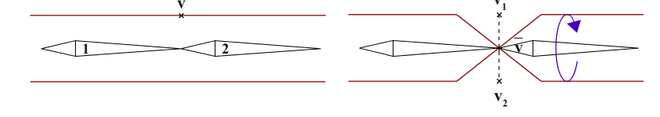
\includegraphics[width=11cm]{01_Skinning/pics/rotationsartefakt.png}
	\caption[Volumenverlust bei Rotation in LBS]{Darstellung des Volumenverlust bei Linear Blend Skinning. Da die beiden Punkte mit gleichen Gewicht an beiden Knochen h�ngen reduzieren sie sich auf einen Punkt. Entnommen von \cite{weights}}
	\label{weights_fig1}
\end{figure}